\documentclass[a4paper,11pt]{article}
\input{/home/tof/Documents/Cozy/latex-include/preambule_doc.tex}
\input{/home/tof/Documents/Cozy/latex-include/preambule_commun.tex}
\newcommand{\showprof}{show them}  % comment this line if you don't want to see todo environment
\setlength{\fboxrule}{0.8pt}
\fancyhead[L]{\fbox{\Large{\textbf{ResSoc 01}}}}
\fancyhead[C]{\textbf{Des réseaux sociaux}}
\newdate{madate}{10}{09}{2020}
%\fancyhead[R]{\displaydate{madate}} %\today
\fancyhead[R]{Seconde - SNT}
%\fancyhead[R]{Première - NSI}
%\fancyhead[R]{Terminale - NSI}
\fancyfoot[L]{\vspace{1mm}Christophe Viroulaud}
\AtEndDocument{\label{lastpage}}
\fancyfoot[C]{\textbf{Page \thepage/\pageref{lastpage}}}
\fancyfoot[R]{\includegraphics[width=2cm,align=t]{/home/tof/Documents/Cozy/latex-include/cc.png}}

\begin{document}
\section{Problématique}
L'évolution rapide du web fait émerger de nouvelles pratiques. Des premiers réseaux de partage apparaissent rapidement:
\begin{itemize}
    \item Classmates en 1995 qui permet de communiquer avec ses anciens camarades de classe,
    \item Linkedin en 2002, qui est orienté sur la vie professionnelle.
\end{itemize}
\begin{center}
\shadowbox{\parbox{10cm}{\centering Peut-on catégoriser les différents réseaux sociaux?}}
\end{center}
\section{Quelles sont mes connaissances?}
\begin{activite}
Pour ceux qui ne l'ont pas déjà fait, réaliser le parcours PIX donné par le professeur. 
\end{activite}
\section{Différents réseaux sociaux}
\begin{activite}
Construire une classe mentale des différents réseaux sociaux, en s'inspirant du modèle ci-dessous (figure \ref{reseau}). Trouver les informations en s'aidant du web. \textbf{Le modèle ci-dessous n'est pas complet, il est juste présenté à titre indicatif.}

Pour construire la carte, utiliser l'application \emph{Carte mentale} du Lycée connecté.
\begin{center}
    \centering
    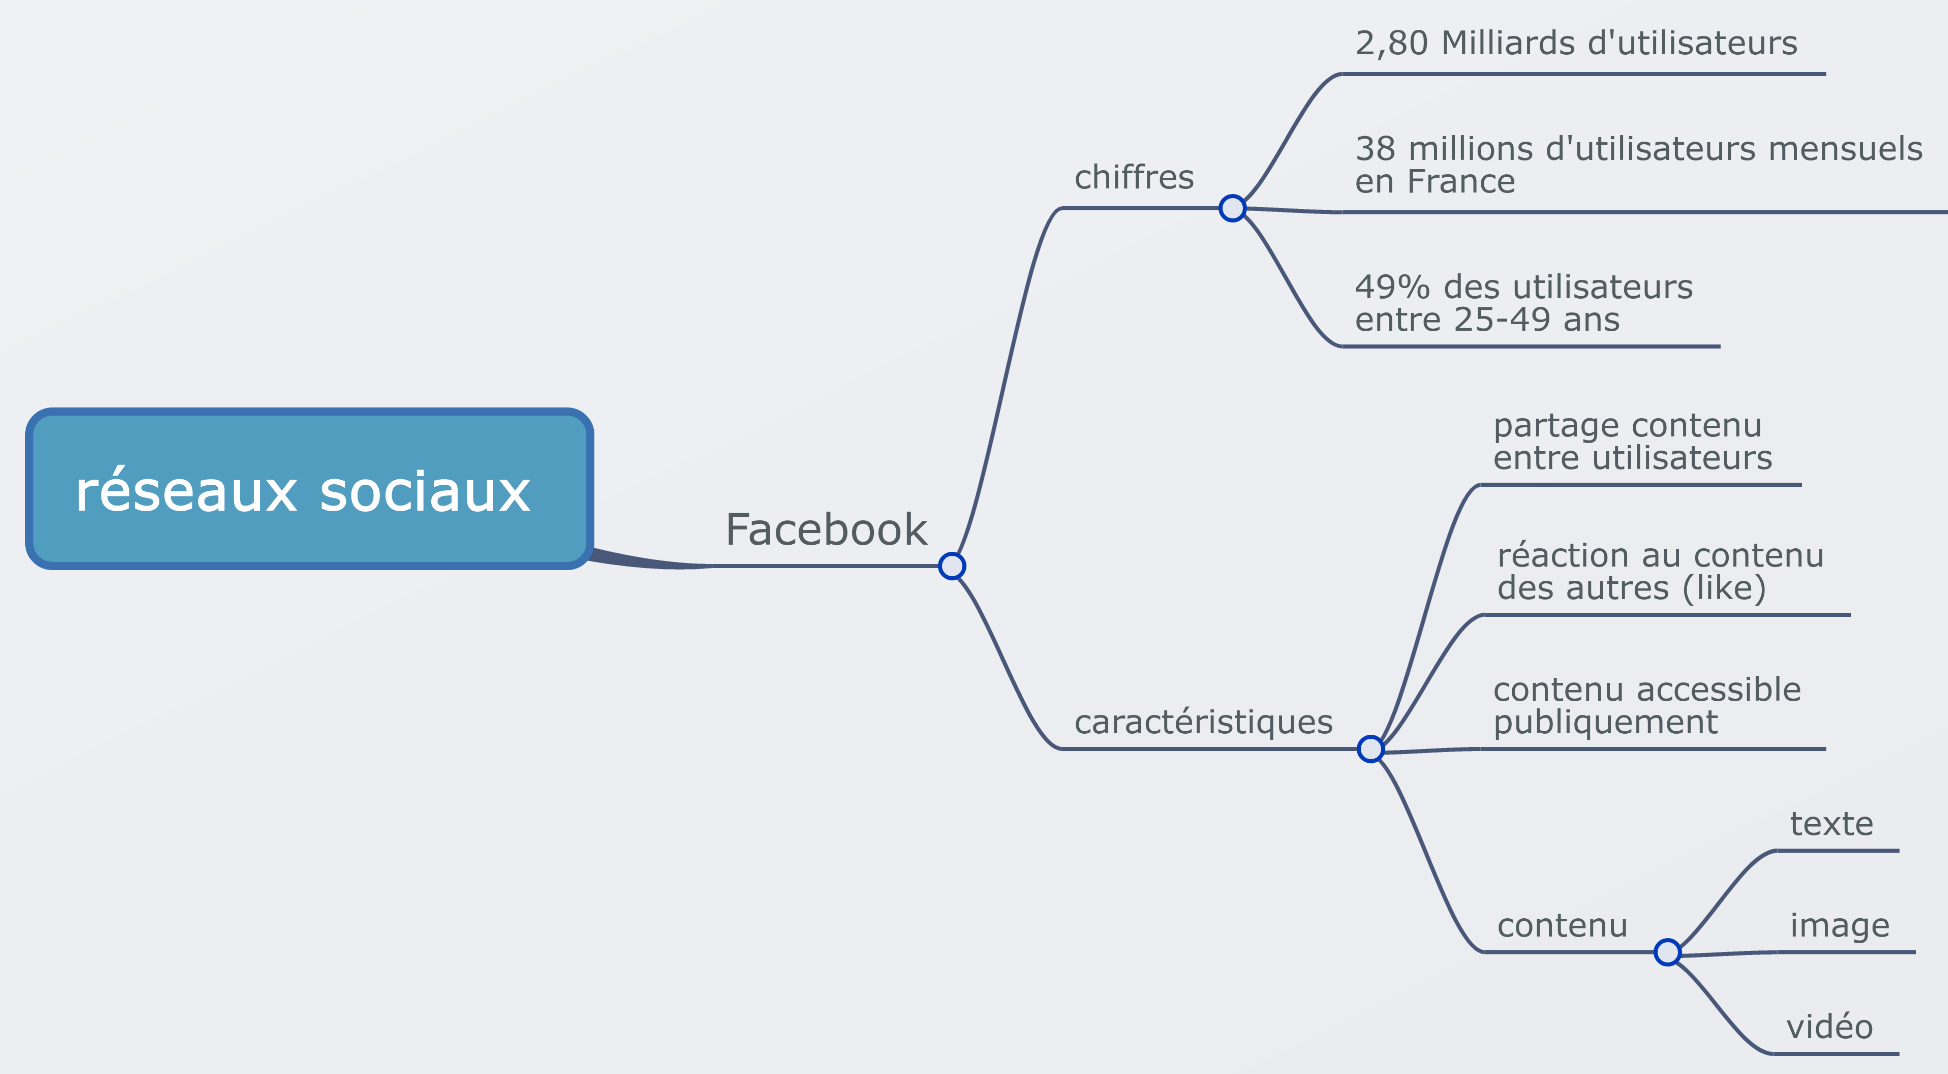
\includegraphics[width=15cm]{ressources/carte-mentale.png}
    \captionof{figure}{Carte mentale}
    \label{reseau}
\end{center}
\end{activite}
\end{document}